\section{Hasil}
\label{sec:results}

\input{generated/leaderboard\langsuffix}

\subsection{Model-model teratas tidak berbeda signifikan}
Tabel~\ref{tab:leaderboard} mengurutkan \NModels{} model menurut skor keseluruhan mereka. \TopName{} memimpin dengan \TopScore{}. Dalam bootstrap terstratifikasi per tugas (Bagian~\ref{sec:setup}), selisih berpasangan terhadap model teratas adalah \DiffB{} [\DiffBLo{}, \DiffBHi{}] untuk \SecondName{}, \DiffC{} [\DiffCLo{}, \DiffCHi{}] untuk \ThirdName{} dan \DiffD{} [\DiffDLo{}, \DiffDHi{}] untuk \FourthName{}. Dengan demikian ketiga model teratas tidak berbeda signifikan, tetapi itu tidak berarti setara: \TopName{} berada di tempat pertama dalam \PTopA{}\,\% dari sampel bootstrap, \SecondName{} dalam \PTopB{}\,\% dan \ThirdName{} dalam \PTopC{}\,\%. Kedekatan mereka sebagian merupakan efek batas atas, karena dua dari delapan tugas hampir tidak membedakan model API (Bagian~\ref{sec:separates}). Di bawahnya model API membentuk pita padat hingga \WorstApiName{} (\WorstApiScore{}); sepuluh model lokal menyusul setelah selisih yang lebar (Bagian~\ref{sec:local}).

\subsection{Biaya}
\begin{figure}[t]
  \centering
  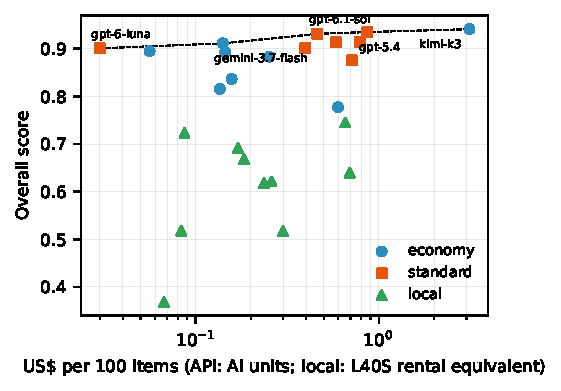
\includegraphics[width=\columnwidth]{pareto}
  \caption{Skor keseluruhan terhadap biaya per 100 butir (skala log; API: AI units pada US\$0.01; lokal: waktu GPU dengan harga on-demand L40S). Garis putus menghubungkan model-model yang tidak dikalahkan oleh model lain pada biaya yang sama atau lebih rendah.}
  \label{fig:pareto}
\end{figure}

Model-model teratas berdekatan dalam kualitas, tetapi tidak dalam harga. Per 100 butir, \TopName{} berharga US\$\TopUSD{}, \SecondName{} US\$\SecondUSD{}, \ThirdName{} US\$\ThirdUSD{} dan \FourthName{} US\$\FourthUSD{}. \CheapName{} mencapai \CheapScore{}, \CheapGap{} di bawah model teratas, dengan US\$\CheapUSD{}, \CostRatio{} kali lebih murah daripada \TopName{}. \ParetoN{} model membentuk front biaya--kualitas (Gbr.~\ref{fig:pareto}): \ParetoNames{}. Harga tidak mengikuti tier yang kami tetapkan berdasarkan nama model: \TopName{}, yang digolongkan bersama model-model hemat, adalah yang paling mahal per butir karena melakukan reasoning panjang (median \TopMedS{}\,s per panggilan terhadap \ThirdMedS{}\,s untuk \ThirdName{}). Seluruh studi menghabiskan US\$\StudyUSD{} untuk panggilan API---US\$\AnswerUSD{} untuk jawaban, US\$\JudgeUSD{} untuk penilaian mereka dan US\$\ProbeUSD{} untuk menguji model-model premium pada dua butir masing-masing---dan \GpuHours{} jam-GPU untuk model lokal.

\subsection{Apa yang membedakan model-model tersebut}
\label{sec:separates}
\input{generated/diagnostics\langsuffix}

Bukan dua tugas yang menuntut pengetahuan, yang mendekati batas atas untuk model API: semua \NApi{} menjawab setidaknya \MethApiMin{} dari pertanyaan metodologi dengan benar, dan \LangCeil{} di antaranya memperoleh skor setidaknya 0.95 pada bahasa Indonesia baku (terendah \LangApiMin{}). Ini menunjukkan bahwa butir-butir ini terlalu mudah bagi model API, bukan bahwa model-model tersebut mengetahui hal yang sama. Tugas-tugas yang menghasilkan artefak membedakan mereka (Tabel~\ref{tab:diagnostics}).

\paragraph{Rujukan} Sebaran terluas di antara model API terdapat pada tugas rujukan (\RefApiMin{}--\RefApiMax{}). Dari rujukan yang dicantumkan model API, \HalApiMin{}--\HalApiMax{}\,\% tidak ditemukan di Crossref, dan banyak yang ditemukan memiliki DOI yang salah: proporsi rujukan yang dicantumkan dengan DOI benar berkisar dari \DoiApiMin{} hingga \DoiApiMax{}\,\%. Audit memperjelas kegagalan tersebut. Dari \AuditApiNF{} rujukan model API yang tidak dikenal Crossref, \AuditApiExact{}\,\% ada yang cocok pada judul, tahun, dan penulis pertama di sumber lain---karya yang terlewat oleh skor yang hanya memakai Crossref---, \AuditApiTitle{}\,\% hanya cocok pada judul dari karya nyata (tahun atau penulis salah, atau judul generik yang kebetulan sama), dan \AuditApiNone{}\,\% tidak ditemukan di mana pun; untuk \AuditLocNF{} kegagalan model lokal, proporsinya adalah \AuditLocExact{}, \AuditLocTitle{} dan \AuditLocNone{}\,\%. Lintasan pertama audit mengungkap dua jebakan Crossref yang kini ditangani oleh aturan (subjudul terpisah, tanggal online-first). Per model, \NoneApiMin{}--\NoneApiMax{}\,\% dari rujukan yang dicantumkan model API tidak ditemukan di mana pun (Gambar~\ref{fig:references}). Memberikan kredit pada karya yang ditemukan audit seperti yang dilakukan pemberi skor akan menaikkan skor rujukan paling banyak sebesar \VerRefMaxGain{} dan membuat peringkat hampir tidak berubah (Spearman $\rho=\VerRho{}$, pergeseran peringkat terbesar \VerMaxShift{}). Model juga berbeda dalam kehati-hatian: gpt-5-mini mencantumkan \RefsGptFiveMini{} rujukan per butir, \NoneGptFiveMini{}\,\% di antaranya tidak ditemukan di mana pun, gemini-3.7-flash selalu mencantumkan lima (\NoneGeminiThreeSevenFlash{}\,\%), dan \TopName{} lima (\NoneKimiKThree{}\,\%). Karena skor memperlakukan abstensi sama dengan rujukan yang tidak dapat diverifikasi, model yang berhati-hati tidak diberi penghargaan karena mencantumkan lebih sedikit; proporsi yang tidak ditemukan di mana pun adalah angka yang perlu diperhatikan demi keamanan.

\begin{figure}[t]
  \centering
  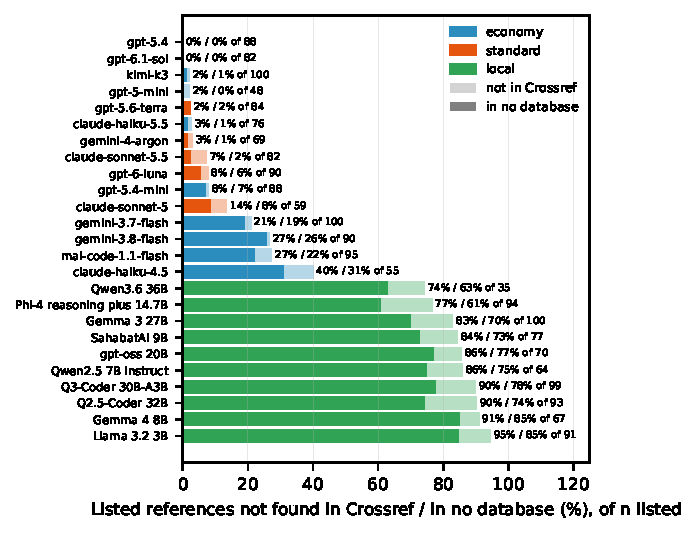
\includegraphics[width=\columnwidth]{references}
  \caption{Proporsi rujukan yang tercantum yang tidak ditemukan di Crossref (terang) dan yang tidak ditemukan di Crossref, doi.org, Scopus, maupun OpenAlex (gelap), beserta jumlah rujukan yang dicantumkan setiap model untuk 20 topik (maksimal 100).}
  \label{fig:references}
\end{figure}

\paragraph{Kerangka} Kerangka bab mendapat skor \StructApiMin{}--\StructApiMax{} untuk model API. Ketidaksesuaian yang sering terjadi adalah bab hasil yang berfokus pada uji: \GenericApiMin{}--\GenericApiMax{}\,\% dari kerangka API menyusun bab~IV di seputar uji asumsi, instrumen, atau hipotesis untuk program studi yang skripsinya tidak menyusun hasilnya dengan cara tersebut.

\paragraph{Kode dan LaTeX} \ApiPerfectCode{} dari \NApi{} model API menyelesaikan setiap tugas pengodean dengan program pertama mereka. Memperbaiki dokumen LaTeX yang rusak lebih sulit daripada menyusun tabel atau entri BibTeX, tugas yang semuanya dilakukan model API dengan benar: model API terlemah menghasilkan dokumen yang dapat dikompilasi hanya untuk \FixApiMin{} dari dokumen yang rusak tersebut.

\paragraph{Penulisan berlandaskan sumber} Berdasarkan pemeriksaan deterministik, model API mematuhi sumber yang diberikan: paling banyak \UnsupApiMax{} angka per ulasan tidak terdapat dalam sumber mana pun, dan sitasi penulis--tahun, yang dilarang oleh tugas, muncul pada paling banyak \ForeignApiMax{}\,\% dari ulasan mereka. Beberapa model lokal mengabaikan format sitasi (sitasi penulis--tahun pada hingga \ForeignLocMax{}\,\% dari ulasan mereka).

\subsection{Model lokal}
\label{sec:local}
\begin{figure}[t]
  \centering
  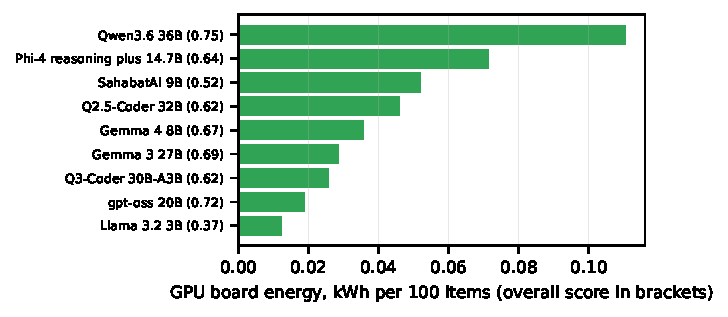
\includegraphics[width=\columnwidth]{energy}
  \caption{Energi papan GPU per 100 butir dari model lokal (kotor; server bersama; Qwen2.5 7B tidak diukur), dengan skor keseluruhan dalam tanda kurung.}
  \label{fig:energy}
\end{figure}

Model lokal terbaik, \BestLocalName{} (\BestLocalScore{}), tetap di bawah model API terlemah, \WorstApiName{} (\WorstApiScore{}). Di antara rata-rata kelompok, selisih terbesar terdapat pada rujukan (\GapRef{}) dan kode (\GapCode{}), lebih kecil pada metodologi (\GapMeth{}) dan paling kecil pada bahasa Indonesia baku (\GapLang{}): model lokal menulis bahasa Indonesia baku pada \LocLangMin{}--\LocLangMax{}, dan Qwen3.6 36B memperoleh skor \TMethodologyQwenThreeSix{} pada pertanyaan metodologi. Dari rujukan yang dicantumkan model lokal, \NoneLocMin{}--\NoneLocMax{}\,\% tidak ditemukan di mana pun, dan mereka menyelesaikan \LocPassOneMin{}--\LocPassOneMax{} dari tugas pemrograman dengan program pertama mereka (rata-rata \LocPassOneMean{}, naik menjadi \LocRepairMean{} setelah satu kali perbaikan). SahabatAI 9B yang disesuaikan untuk bahasa Indonesia memperoleh skor bahasa Indonesia baku lebih rendah daripada Gemma~4 8B umum (\SahLang{} berbanding \GemmaFourLang{}) dan gagal pada kode (\SahCode{}), sehingga skor keseluruhannya (\SahOverall{}) tetap di bawah Gemma~4 (\GemmaFourOverall{}). Dengan harga on-demand L40S dan tiga permintaan paralel, biaya model lokal mencapai US\$\LocUSDMin{}--\LocUSDMax{} per 100 butir, tidak kurang dari model API termurah, dan mengonsumsi \LocKwhMin{}--\LocKwhMax{}\,kWh per 100 butir (Gambar~\ref{fig:energy}); gpt-oss 20B memberikan skor paling tinggi per kWh dalam konfigurasi ini (\ScoreGptOss{} untuk \KwhGptOss{}\,kWh dan US\$\UsdGptOss{} per 100 butir).

\subsection{Juri dan provenans}
Ketiga juri menilai \NJudgedAnswers{} jawaban dengan \NJudgeCalls{} penilaian. Pada \NAllJudges{} jawaban yang dinilai ketiganya (kandidat dari vendor selain para juri), rata-rata penilaian mereka sepakat dengan $\alpha$ Krippendorff sebesar \AlphaJudges{} (interval); kriteria tunggal lebih rendah kesesuaiannya ($\alpha$ dari \AlphaCritMin{} sampai \AlphaCritMax{}, ordinal), paling rendah untuk kepatuhan instruksi dan kesetiaan. Kelunakan para juri berbeda hingga \LeniencyRange{} pada skala 0--1, yang dikoreksi oleh kalibrasi. Skor mereka mengikuti pemeriksaan deterministik: $\rho$ Spearman bernilai \RhoAnsGrd{} (berlandaskan sumber) dan \RhoAnsLng{} (bahasa) di seluruh jawaban, serta \RhoModelGrd{} dan \RhoModelLng{} di seluruh rata-rata model. Panel ekstraksi sepakat secara bulat pada \SilverUnanimous{}\,\% dari bidang; teknik analisis merupakan bidang tersulit (tidak ada mayoritas pada \SilverAnalysisNone{} dari 30 cuplikan, yang oleh karena itu tidak dinilai). Dalam semua \NApiCalls{} panggilan API studi ini, SDK melaporkan model yang diminta sebagai model yang menjawab: substitusi senyap yang dilaporkan untuk SDK yang sama ketika sebuah akun tidak berhak atas suatu model~\cite{arya2026paperagent} tidak terjadi di sini. Pemeriksaan didasarkan pada peristiwa penggunaan SDK itu sendiri, bukan pada pengujian independen terhadap backend.
